\documentclass[a4paper]{article}

\usepackage[catalan]{babel} % Language 
\usepackage{fontspec}
\usepackage[margin=2cm]{geometry}
\usepackage{float}
\usepackage[dvipsnames]{xcolor}
\usepackage{pgfplots}
\usepackage{pgfplotstable}
\usepackage[hidelinks]{hyperref}
\usepackage{enumitem}
\usepackage{amsmath}
\usepackage{gensymb} % For the degree symbol
\usepackage{graphicx}
\usepackage{longtable}
\usepackage{multirow}
\usepackage{array}
\usepackage{multicol}

\setlength{\parindent}{0pt}
\setlength{\parskip}{1em}

\newcolumntype{R}{>{\raggedleft}p{2cm}}

\title{Projecte APA}
\author{Joan Marcè \and Esteve Tarragó}

\begin{document}
\maketitle
\tableofcontents
\newpage

\section{Introducció}

En aquest treball s'ha de realitzar una aplicació pràctica dels diferents coneixements de \emph{Machine Learning} adquirits a classe. Així doncs, s'ha escollit un conjunt de dades per realitzar una aplicació pràctica mitjançant mètodes de classificació. 

El conjunt de dades escollit ha estat \emph{Grammatical Facial Expressions Data Set}. Aquests han estat obtinguts mitjançant una càmera \emph{Kinect} que ha enregistrat diferents punts (100) en tres dimensions de la cara de diverses persones al llarg del temps mentre realitzen una paraula en el llenguatge de signes brasiler. Aquestes expressions van combinades amb gestos amb la mà però en aquest cas només s'ha gravat la cara. Després, aquests conjunts han estat analitzats manualment per decidir quins fotogrames estan fent realment una expressió facial i quins no. 

Les dades es poden obtenir en el següent enllaç:  \url{http://archive.ics.uci.edu/ml/datasets/Grammatical+Facial+Expressions}

A part, aquestes dades també s'han usat en treballs anteriors \cite{freitas}.

\begin{figure}[H]
	\centering
	\fbox{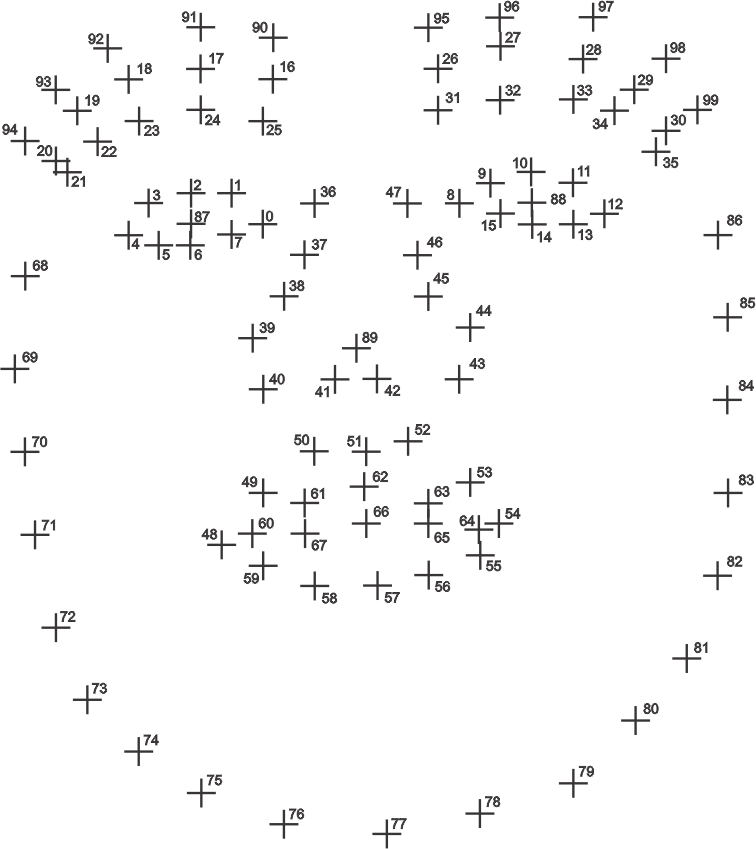
\includegraphics[width=0.6\textwidth]{images/view_points}}
	\caption{Representació dels punts de la cara que són utilitzats en la presa de dades}
\end{figure}

\section{Objectius}

L'objectiu d'aquest treball és poder decidir a partir d'una dada no usada prèviament:
\begin{enumerate}
	\item A partir d'una sola expressió facial si aquella s'està realitzant o no.
	\item A partir de tot el conjunt de dades si s'està realitzant o no una expressió facial.
	\item En el cas en el que s'estigui realitzant una expressió facial, poder decidir de quin tipus d'expressió facial (o paraula) es tracta.
	\item Trobar quin tipus de model s'adequa millor als objectius anteriors i comprar-los entre ells.
\end{enumerate}

\section{Procés d'exploració de dades}

S'han realitzat dos \emph{scripts} en R. El primer és per visualitzar les dades cronològicament (\verb|loadData.R|) i el segon és per poder interpretar-les a l'hora de realitzar una classificació (\verb|clustering.R|).

En aquest cas interessa més el segon ja que és el que tracta el problema de \emph{clustering}. S'han realitzat dos tipus d'algoritmes\cite{bishop} per projectar les dades, FDA i PCA. L'\emph{script} requereix que es seleccioni primerament quina expressió (\verb|*_datapoints.txt|) i a continuació quins resultats (\verb|*_targets.txt|) es volen agafar. També cal introduir de quin punt es volen visualitzar les dades (variable \verb|point|). 

A continuació es mostren els resultats obtinguts amb el conjunt de dades \verb|a_affirmative_datapoints.txt| i \verb|a_affirmative_targets.txt| i el punt 60 que correspon a la part superior del llavi. Per representar les dades s'han restat les mitjanes per tal que tant els punts com la recta de projecció estiguin centrades al voltant de $(0,0)$.

\begin{longtable}{cc}
	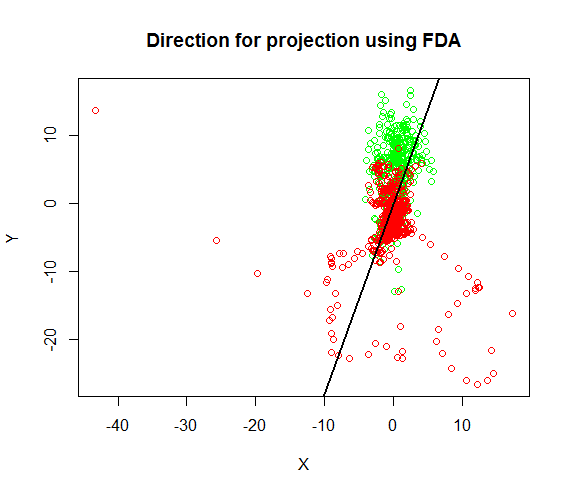
\includegraphics[width=0.45\textwidth]{images/FDA_XY} &
	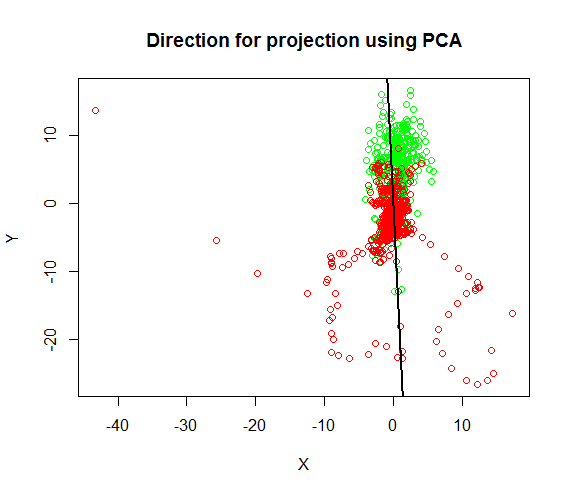
\includegraphics[width=0.45\textwidth]{images/PCA_XY} \\
	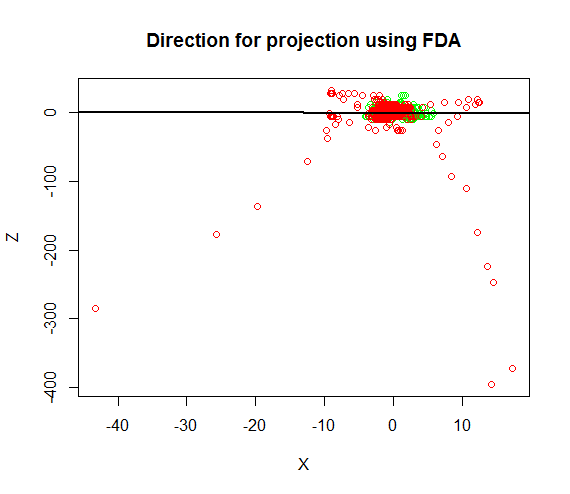
\includegraphics[width=0.45\textwidth]{images/FDA_XZ} &
	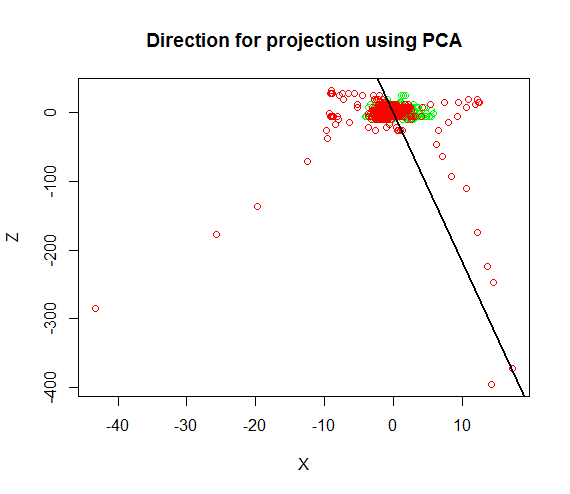
\includegraphics[width=0.45\textwidth]{images/PCA_XZ} \\
	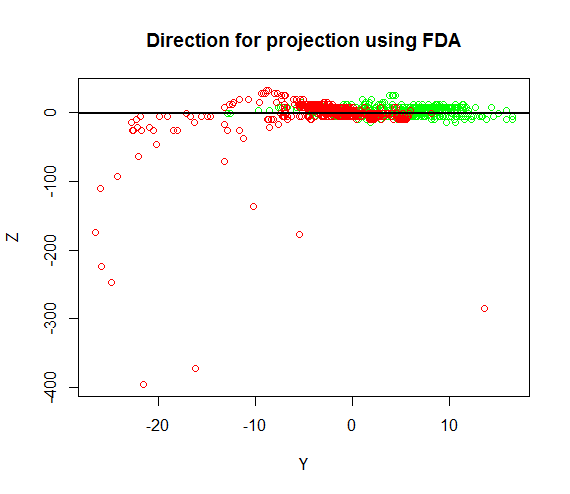
\includegraphics[width=0.45\textwidth]{images/FDA_YZ} &
	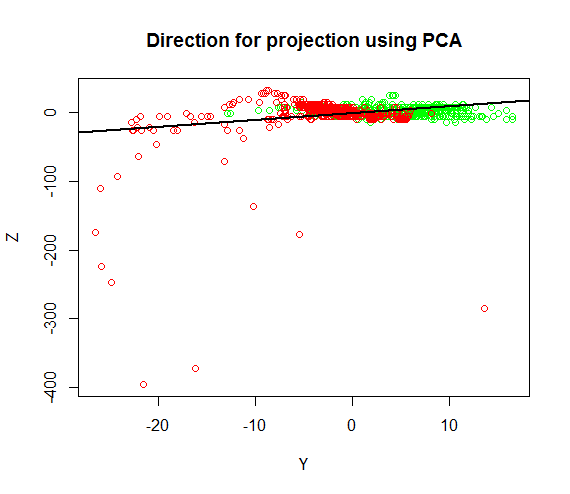
\includegraphics[width=0.45\textwidth]{images/PCA_YZ} \\
	\multicolumn{2}{c}{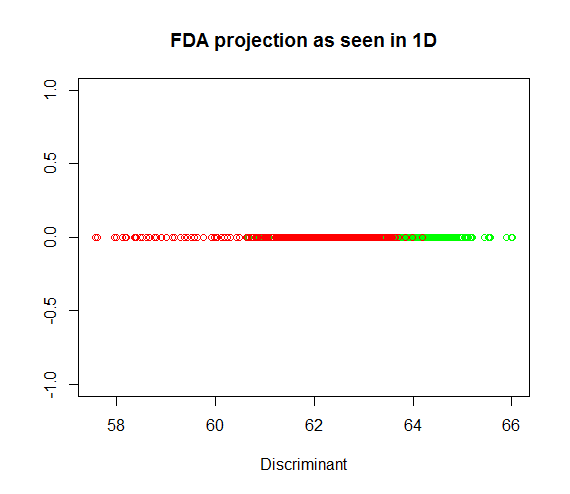
\includegraphics[width=0.5\textwidth]{images/FDA_projection}}
\end{longtable}

Com es pot veure als gràfics anteriors la dada Z no permet agrupar les dades gaire bé ja que totes queden al voltant dels valors \verb|Z = 0|. Tot i així es pot veure en les dimensions $X$ i $Y$ la separació de les dades es relativament fàcil. 

També, donat que sembla ser viable una projecció, es pot fer una projecció de cada punt de 3 dimensions a una sola dimensió. Això és el que s'ha fet a l'script \texttt{reduceData.R} de manera que cada punt és projectat a una sola dimensió reduint l'espai de dades de 300 dimensions a 100 dimensions. Tot i així hi ha una pèrdua d'informació al fer la projecció però s'ha considerat que aquesta pèrdua d'informació és poca en comparació al guany que s'obté al reduir les dimensions.

\section{Resultats amb mètodes lineals/quadràtics}
Donat que hi ha diversos objectius en aquest treball s'han usat diferents mètodes per a poder resoldre cadascun dels objectius, han estat els següents:
\begin{itemize}
	\item Regressió logística i LDA:
	\begin{itemize}
		\item A partir d'una sola expressió facial si aquella s'està realitzant o no.
		\item A partir de tot el conjunt de dades si s'està realitzant o no una expressió facial.
	\end{itemize}
	\item QDA i LDA:
	\begin{itemize}
		\item En el cas en el que s'estigui realitzant una expressió facial, poder decidir de quin tipus d'expressió facial (o paraula) es tracta.
	\end{itemize}
\end{itemize}

\subsection{Detecció d'expressió facial}
\subsubsection{Regressió Logística}
L'script \verb|logistic.R| realitza classificació amb regressió logística mitjançant l'ajuda de \verb|glm|. Per poder utilitzar l'script cal posar el \verb|Working Directory| a l'arrel de la carpeta subministrada i un cop es comença a executar cal escollir les dades que es volen usar per entrenar i les que es volen usar per validar. Inicialment s'havia decidit usar les dades dels arxius \verb|a_*.txt| per entrenar i les dels \verb|b_*.txt| per validar les dades tot i que això no aporta bons resultats. A continuació es pot comparar l'error entre utilitzar un sol conjunt per entrenar i usar un subconjunt de totes les dades.

En el primer experiment s'han usat totes les expressions facials d'una persona (dades contingudes a tots els arxius \verb|a_*.txt|) per a l'entrenament i per a la validació s'han usat totes les dades de l'altre persona (dades contingudes a tots els arxius \verb|b_*.txt|). Es poden veure els resultats a la \autoref{tab:reglog_training1} i la \autoref{tab:reglog_training2}.

\begin{table}[H]
	\centering
	\def\arraystretch{1.5}
	\begin{tabular}{c|rr}
		& \multicolumn{2}{c}{Valor real} \\
		Valor predit & 0 & 1 \\
		\hline
		0 & 8912 & 361 \\
		1 & 242 & 4095 \\
	\end{tabular}
	\caption{Valors predits pel conjunt d'entrenament. L'error és d'un 4,43\%.}
	\label{tab:reglog_training1}
\end{table}

\begin{table}[H]
	\centering
	\def\arraystretch{1.5}
	\begin{tabular}{c|rr}
		& \multicolumn{2}{c}{Valor real} \\
		Valor predit & 0 & 1 \\
		\hline
		0 & 5725 & 2962 \\
		1 & 3180 & 2459 \\
	\end{tabular}
	\caption{Valors predits pel conjunt de validació. L'error és d'un 42,87\%.}
	\label{tab:reglog_training2}
\end{table}

En aquest segon experiment s'ha usat un subconjunt de totes les dades per entrenar i el complementari d'aquest per validar les dades, com es pot observar a la \autoref{tab:reglog_training4} s'obtenen millors resultats per les dades de validació respecte \autoref{tab:reglog_training2}.

\begin{table}[H]
	\centering
	\def\arraystretch{1.5}
	\begin{tabular}{c|rr}
		& \multicolumn{2}{c}{Valor real} \\
		Valor predit & 0 & 1 \\
		\hline
		0 & 2306 & 543 \\
		1 &  247 & 894 \\
	\end{tabular}
	\caption{Valors predits pel conjunt d'entrenament. L'error és d'un 19,8 \%.}
	\label{tab:reglog_training3}
\end{table}

\begin{table}[H]
	\centering
	\def\arraystretch{1.5}
	\begin{tabular}{c|rr}
		& \multicolumn{2}{c}{Valor real} \\
		Valor predit & 0 & 1 \\
		\hline
		0 & 13914 & 3147 \\
		1 &  1592 & 5293 \\
	\end{tabular}
	\caption{Valors predits pel conjunt de validació. L'error és d'un 19,79 \%.}
	\label{tab:reglog_training4}
\end{table}

\subsubsection{LDA}
L'script \verb|LDA_si_no.R| realitza classificació amb \emph{lda} mitjançant l'ajuda de \verb|lda|. Per poder utilitzar l'script cal posar el \verb|Working Directory| a l'arrel de la carpeta subministrada i un cop es comença a executar cal escollir les dades que es volen usar. 
 
En el primer experiment s'han usat totes les expressions facials d'una persona (dades contingudes a tots els arxius \verb|a_*.txt|) per a l'entrenament i per a la validació s'han usat totes les dades de l'altre persona (dades contingudes a tots els arxius \verb|b_*.txt|). Es poden veure els resultats a la \autoref{tab:lda_yes_no1} i la 	\autoref{tab:lda_yes_no2}.

\begin{table}[H]
	\centering
	\def\arraystretch{1.5}
	\begin{tabular}{c|rr}
		& \multicolumn{2}{c}{Valor real} \\
		Valor predit & 0 & 1 \\
		\hline
		0 & 8876 & 459 \\
		1 & 278 & 3997 \\
	\end{tabular}
	\caption{Valors predits pel conjunt d'entrenament. L'error és d'un 5,42\%.}
	\label{tab:lda_yes_no1}
\end{table}

\begin{table}[H]
	\centering
	\def\arraystretch{1.5}
	\begin{tabular}{c|rr}
		& \multicolumn{2}{c}{Valor real} \\
		Valor predit & 0 & 1 \\
		\hline
		0 & 5018 & 2317 \\
		1 & 3887 & 3104 \\
	\end{tabular}
	\caption{Valors predits pel conjunt de validació. L'error és d'un 43,31\%.}
	\label{tab:lda_yes_no2}
\end{table}

En aquest segon experiment s'ha usat un subconjunt de totes les dades per entrenar i el complementari d'aquest per validar les dades, com es pot observar a la \autoref{tab:lda_yes_no4} s'obtenen millors resultats per les dades de validació.

\begin{table}[H]
	\centering
	\def\arraystretch{1.5}
	\begin{tabular}{c|rr}
		& \multicolumn{2}{c}{Valor real} \\
		Valor predit & 0 & 1 \\
		\hline
		0 & 4088 & 1034 \\
		1 &  414 & 1448 \\
	\end{tabular}
	\caption{Valors predits pel conjunt d'entrenament. L'error és d'un 20,73 \%.}
	\label{tab:lda_yes_no3}
\end{table}

\begin{table}[H]
	\centering
	\def\arraystretch{1.5}
	\begin{tabular}{c|rr}
		& \multicolumn{2}{c}{Valor real} \\
		Valor predit & 0 & 1 \\
		\hline
		0 & 12334 & 3036 \\
		1 &  1223 & 4359 \\
	\end{tabular}
	\caption{Valors predits pel conjunt de validació. L'error és d'un 20,33 \%.}
	\label{tab:lda_yes_no4}
\end{table}

\subsection{Detecció de tipus d'expressió}
\subsubsection{LDA}

L’script \verb|LDA_K.R|  obté un model LDA i a continuació testeja el model mitjançant cross-validation i aplicant-lo a un altre subjecte.

Els resultats obtinguts son oposats. Això ens indica que hi ha fortes diferències entre els les expressions de ambdues persones exceptuant la expressió condicional que obté un un error molt reduït en comparació a la resta d’expressions.

També destaca que les expressions de afirmació s’han classificat com a èmfasis majoritàriament i viceversa. Això podria indicar que la persona B i la A tenen les expressions de èmfasis i afirmació invertides.

\begin{table}[H]
	\centering
	\begin{tabular}{c|rrrrrrrrrr}
		& \multicolumn{10}{c}{Valor real} \\
		 & 1 & 2 & 3 & 4 & 5 & 6 & 7 & 8 & 9 & 10 \\
		 \hline
		1 & 8626 & 61 & 22 & 67 & 26 & 57 & 35 & 42 & 40 & 40 \\
		2 & 98 & 353 & 4 & 3 & 1 & 3 & 2 & 1 & 0 & 3 \\
		3 & 45 & 0 & 497 & 10 & 2 & 3 & 0 & 1 & 0 & 3 \\
		4 & 43 & 0 & 4 & 372 & 2 & 2 & 1 & 1 & 0 & 5 \\
		5 & 25 & 0 & 2 & 5 & 295 & 5 & 0 & 1 & 0 & 0 \\
		6 & 66 & 0 & 4 & 6 & 0 & 448 & 0 & 1 & 0 & 2 \\
		7 & 49 & 0 & 4 & 3 & 1 & 2 & 602 & 1 & 0 & 5 \\
		8 & 44 & 0 & 5 & 5 & 1 & 1 & 2 & 311 & 0 & 3 \\
		9 & 98 & 0 & 3 & 11 & 0 & 2 & 1 & 1 & 569 & 1 \\
		10 & 60 & 0 & 3 & 9 & 2 & 5 & 1 & 0 & 0 & 470 \\
	\end{tabular}
	\caption{Resultats obtinguts a l'usar cross-validation. Error total 8\%.}
\end{table}

\begin{figure}[H]
	\centering
	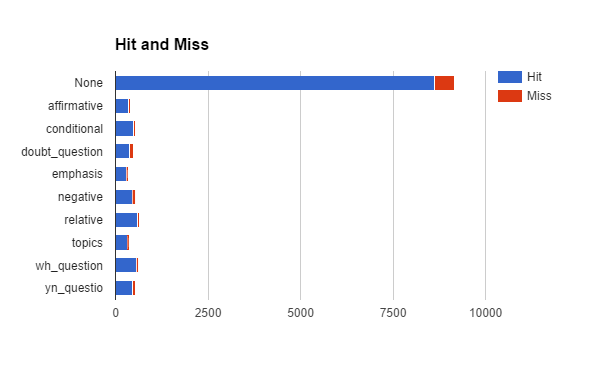
\includegraphics[width=\textwidth]{images/image00}
\end{figure}

\begin{table}[H]
	\centering
	\begin{tabular}{c|rrrrrrrrrr}
		& \multicolumn{10}{c}{Valor real} \\
		& 1 & 2 & 3 & 4 & 5 & 6 & 7 & 8 & 9 & 10 \\
		\hline
		1 & 8 & 0 & 0 & 0 & 1 & 0 & 0 & 0 & 0 & 0\\
		2 & 855 & 2 & 0 & 65 & \textcolor{Orange}{349} & 0 & 14 & 0 & 21 & 137\\
		3 & 1393 & 0 & 554 & 0 & 27 & 6 & 0 & 0 & 3 & 0\\
		4 & 182 & 0 & 35 & 74 & 0 & 0 & 0 & 0 & 0 & 9\\
		5 & 3172 & \textcolor{Orange}{526} & 0 & 518 & 0 & 586 & 0 & 465 & 358 & 88\\
		6 & 360 & 0 & 0 & 3 & 0 & 0 & 0 & 0 & 72 & 73\\
		7 & 954 & 0 & 0 & 46 & 72 & 120 & 0 & 0 & 24 & 325\\
		8 & 8 & 0 & 0 & 17 & 82 & 0 & 0 & 1 & 2 & 0\\
		9 & 520 & 0 & 0 & 0 & 0 & 0 & 66 & 0 & 0 & 14\\
		10 & 1453 & 0 & 0 & 57 & 0 & 0 & 470 & 1 & 69 & 69\\
	\end{tabular}
	\caption{Resultats obtinguts al validar les dades amb una altra persona. Error total 95\%}
\end{table}

\begin{figure}[H]
	\centering
	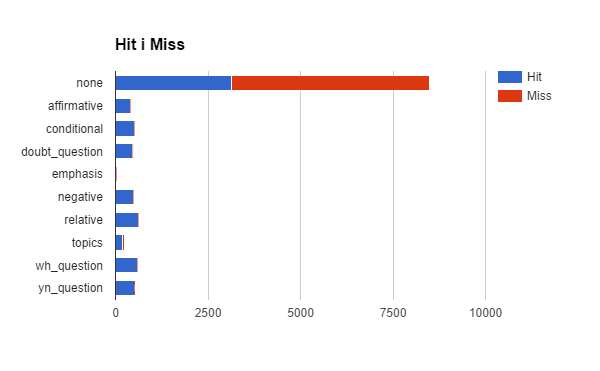
\includegraphics[width=\textwidth]{images/image01}
\end{figure}

\begin{multicols}{3}
	\begin{enumerate}
		\item None 
		\item affirmative 
		\item conditional 
		\item doubt question 
		\item emphasis 
		\item negative 
		\item relative 
		\item topics 
		\item wh question 
		\item yn question
	\end{enumerate}
\end{multicols}

\subsubsection{QDA}
L’script \verb|QDA_K.R|  obté un model QDA i a continuació testeja el model mitjançant cross-validation i aplicant-lo a un altre subjecte.


En comparació amb el LDA podem veure un error molt major alhora de predir les no expressions. També veiem que l’error a l’hora de predir quan s’esta fent una expressió es molt menor que en el LDA exceptuant l’expressió d’emphasis que LDA la categoritza millor

\begin{table}[H]
	\centering
	\begin{tabular}{c|rrrrrrrrrr}
		& \multicolumn{10}{c}{Valor real} \\
		& 1 & 2 & 3 & 4 & 5 & 6 & 7 & 8 & 9 & 10 \\
		\hline
		1 & 3131 & 0 & 0 & 2 & 23 & 0 & 0 & 53 & 0 & 1 \\
		2 & 572 & 409 & 0 & 0 & 0 & 0 & 0 & 0 & 0 & 0 \\
		3 & 850 & 0 & 510 & 0 & 0 & 0 & 0 & 0 & 0 & 0 \\
		4 & 582 & 0 & 0 & 461 & 0 & 0 & 0 & 0 & 0 & 0 \\
		5 & 0 & 0 & 0 & 0 & 4 & 0 & 0 & 0 & 0 & 0 \\
		6 & 541 & 0 & 0 & 0 & 0 & 492 & 0 & 0 & 0 & 0 \\
		7 & 1204 & 0 & 0 & 0 & 0 & 0 & 621 & 0 & 0 & 0 \\
		8 & 196 & 0 & 0 & 0 & 0 & 0 & 0 & 202 & 0 & 0 \\
		9 & 623 & 0 & 0 & 0 & 0 & 0 & 0 & 0 & 605 & 0 \\
		10 & 782 & 0 & 0 & 0 & 0 & 0 & 0 & 0 & 0 & 509 \\
	\end{tabular}
	\caption{Resultats obtinguts al validar les dades amb cross-validation. Error total 43\%}
\end{table}

\begin{figure}[H]
	\centering
	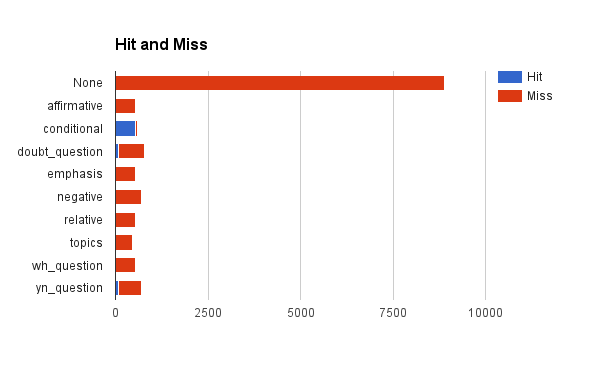
\includegraphics[width=\textwidth]{images/image02}
\end{figure}

Quan s'utilitza un altre individu per validar les dades, totes es prediuen amb sortida \emph{None} per tant aquest model no ens permet extrapolar res tot hi tenir un error total menor (35\%). Es podria dir que el individu B es menys expressiu que l’individu A  en aquest model ja que totes les seves expressions es categoritzen com a \emph{no expressió}.

\section{Resultats amb mètodes no lineals}
\section{Model final escollit}
\section{Conclusions}
\section{Possibles extensions}
\section{Referències}

\bibliographystyle{acm}
\bibliography{bibliography}

\end{document}